% -*- mode: LaTeX; coding: utf-8 -*-
% Typeset with: XeLaTeX

\documentclass{beamer}
\usetheme{Madrid}
\centering

% Greek fonts
\RequirePackage[cm-default]{fontspec}
\defaultfontfeatures{Mapping=tex-text}
  % you may want to try: {FreeSerif} or {Times New Roman}
\setmainfont{Liberation Serif}
  % you may want to try: {FreeSans} or {Arial}
\setsansfont[Scale=MatchLowercase]{Liberation Sans}
  % you may want to try: {FreeMono} or {Courier New}
\setmonofont[Scale=MatchLowercase]{Liberation Mono}

\usepackage{graphicx}
\graphicspath{ {./pr1_figures/} }

% Main document
\begin{document}
\title{DeepSite}
\subtitle{Algorithms in Structural Bioinformatics - Project progress report 1}
\author{Thomas Pappas}
%\date{4 March 2020}
\maketitle

\section{What is the project about?}

\begin{frame}{What is the project about?}
  \begin{block}{DeepSite}
    Protein-binding site predictor using 3D-convolutional neural networks
    \begin{itemize}
      \item Deep Convolutional Neural Network (DCNN)
      \item Trained by 7622 proteins from scPDB
      \item Superior performance to two other competitive algorithmic strategies
      \item Available online at\\ \url{https://www.playmolecule.com/deepsite/}
  \end{itemize}
  \end{block}
\end{frame}

\begin{frame}{Example of a 6FAT protein}
  \begin{figure}[h]
    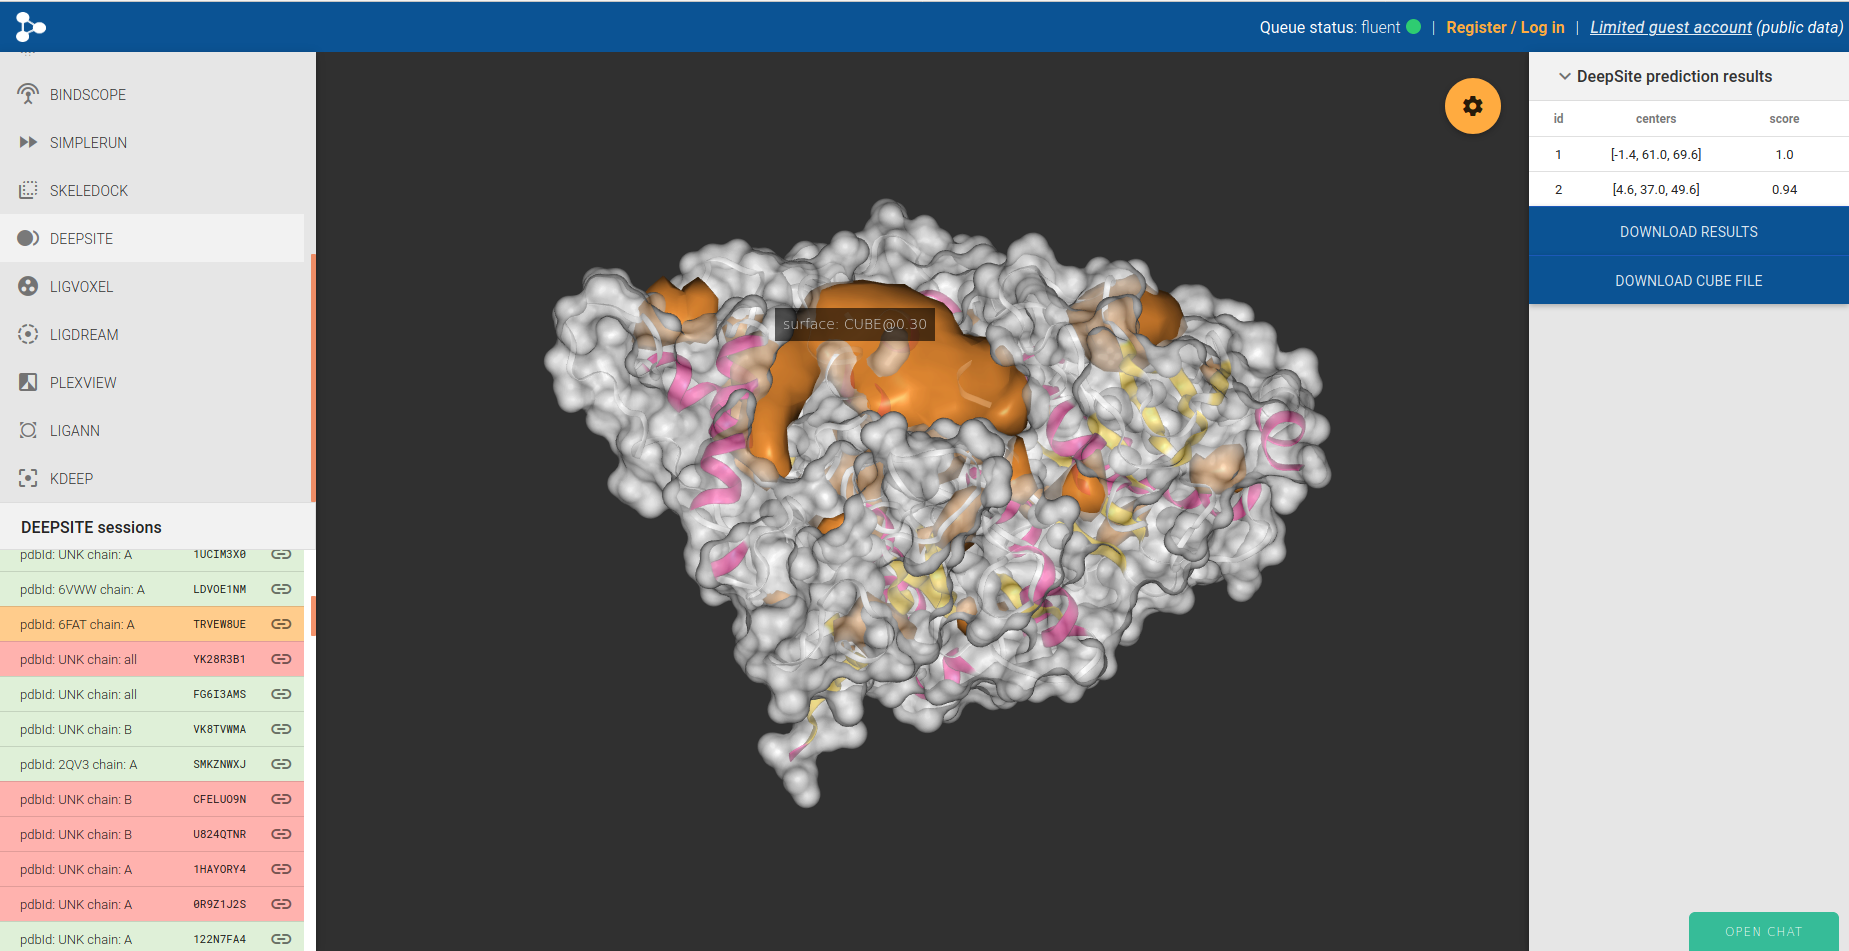
\includegraphics[width=1\textwidth]{deepsite_6fat_result}
    \caption{The 6FAT protein submitted in the \href{https://www.playmolecule.com/deepsite/}{DeepSite web app}}
  \end{figure}
\end{frame}

\subsection{What has happened?}

\begin{frame}{What has happened?}
  \begin{block}{Research}
    \begin{itemize}
      \item Neural Networks
      \item Convolutional Neural Networks
    \end{itemize}
  \end{block}
  \begin{block}{Analysis}
    DCNN for protein binding site prediction
    \begin{itemize}
      \item Treat the 3D protein molecular structure like a 3D image
      \begin{itemize}
        \item $1$ voxel = $1 \times 1 \times 1 $ \AA$^3$
      \end{itemize}
      \item Apply atom properties (hydrophobic, aromatic, etc.) as filters
      \item 10-fold cross-validation
      \item Network design
      \item Evaluation using DCC and DVO (with Jaccard Index)
    \end{itemize}
  \end{block}
\end{frame}

\begin{frame}{The protein property filters}
  \begin{figure}[h]
    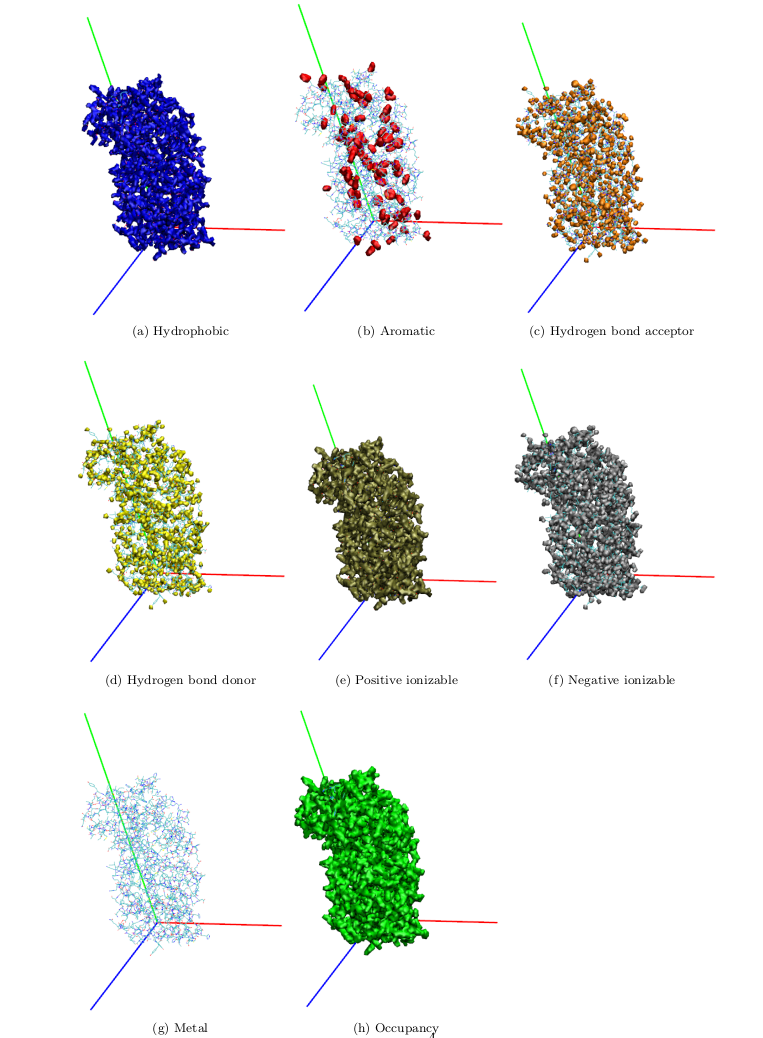
\includegraphics[width=0.4\textwidth]{deepsite_protein_property_filters}
    \caption{The 8 protein properties that contitute the filters of the DCNN.\\\hspace{1mm}
      From the DeepSite 2017 paper, 10.1093/bioinformatics/btx350}
  \end{figure}
\end{frame}

\subsection{What will happen?}

\begin{frame}{What will happen?}
  \begin{block}{Problems}
    The paper does NOT provide the full algorithm, therefore no easy tweaking can take place
  \end{block}
  \begin{block}{More Research}
    \begin{itemize}
      \item DCNN design choices
      \item NN - Binding site problem relation
    \end{itemize}
  \end{block}
  \begin{block}{Investigation suggestions}
    \begin{itemize}
      \item Protein sample submission to online application
      \begin{itemize}
        \item Visualisation
        \item Modify propability threshold
      \end{itemize}
    \end{itemize}
  \end{block}
\end{frame}

\subsection{Contact details}

\begin{frame}{Contact details}
  \begin{center}
    Thomas Pappas\\
    \href{mailto:thpappas@di.uoa.gr}{thpappas@di.uoa.gr}
  \end{center}
\end{frame}

\end{document}
